%% EXHALE (EXHALE): closed-form metal line-cooling formulas.
%% Complete reference for the analytic cooling coefficients implemented in
%% Cool_coeff.f90 (2026-08-12): CHIANTI-fitted resonance lines, Fe II,
%% C/N/O (with the AIOLOS fits for comparison), and the
%% ground-term fine-structure statistical equilibrium of C I/C II/N II/O I.
%% Fit provenance: cooling_data/fit_cooling_formulas.py,
%% fit_cno_formulas.py, fit_fs_saturation.py; figures by
%% cooling_data/make_cooling_doc_figures.py.
%% Author: Kwang-Il Seon
\documentclass[english,a4paper]{my_memo}
\synctex=1
\usepackage{booktabs}
\usepackage{amsmath}
\usepackage{graphicx}
\usepackage{babel}
\emergencystretch=3em

\title{Closed-form metal line-cooling formulas in EXHALE}
\author{Kwang-Il Seon}
%%\date{2026-08-12}
\date{Last updated: \docmoddate}

\begin{document}
\maketitle

\section{Overview and conventions}

All metal line-cooling coefficients in \texttt{Cool\_coeff.f90} are
evaluated from closed-form analytic expressions fitted to the CHIANTI
v11.0.2 database (Burgess--Tully descaled \texttt{.scups} effective
collision strengths); only Fe\,I (1-D) and the density-dependent Fe\,II
statistical-equilibrium coefficient (2-D) remain tabulated.  Throughout,
$\Lambda(T)$ denotes the effective cooling coefficient \emph{per}
$(n_e\,n_{\rm ion})$ in $\mathrm{erg\,cm^3\,s^{-1}}$, in the optically
thin limit (every collisional excitation is followed by a radiative
decay); the cooling assembly multiplies by
$\beta_{\rm esc}\,n_e\,n_{\rm ion}$.  Lower levels are populated in
Boltzmann equilibrium over the ground-term fine structure where one
exists.  Two practical conventions matter when reproducing the numbers:
(i) the fits and every number quoted here were made with the rounded
$k_B = 1.38\times10^{-16}\,\mathrm{erg\,K^{-1}}$, the code-wide value
until 2026-08-15; the code now carries the CODATA
$1.380649\times10^{-16}$ (Update\_EXHALE \S62.2), a $4.7\times10^{-4}$
relative shift that is negligible against the fit errors;
(ii) the transition energies recovered by the fits
are the CHIANTI \texttt{.scups} \emph{theoretical} energies, which can
differ from the observed-wavelength energies by a few percent (e.g.\
Mg\,II $4.277$ vs.\ $4.43$\,eV) --- using the observed value inflates
the fit error from ${\sim}1\%$ to ${\sim}5\%$.

Fit scripts (in \texttt{cooling\_data/}):
\texttt{fit\_cooling\_formulas.py} (resonance lines, Fe\,II),
\texttt{fit\_cno\_formulas.py} (C/N/O),
\texttt{fit\_fs\_saturation.py} (fine-structure saturation).
The companion notebooks \texttt{cooling\_formula\_fits.ipynb} and
\texttt{cno\_cooling\_comparison.ipynb} reproduce every figure here.

\section{Resonance lines: exact two-level skeleton}
\label{sec:resonance}

A single-channel resonance line obeys exactly
\begin{equation}
\Lambda(T) \;=\; \frac{8.629\times10^{-6}}{g_l\,\sqrt{T}}\;
\Upsilon(T)\;\Delta E\;e^{-\Delta E/k_BT},
\label{eq:twolevel}
\end{equation}
so the only quantity to fit is the slowly varying effective collision
strength, for which the Burgess--Tully type-1 asymptotic form
\begin{equation}
\Upsilon(T) \;=\; a + b\,\ln\!\left(1 + T/T_0\right)
\label{eq:btups}
\end{equation}
suffices.  Table~\ref{tab:resonance} lists the fitted constants;
Fig.~\ref{fig:resfits} compares the formulas with the source tables.
Na\,I D is reproduced essentially exactly because the underlying rate
is itself a Van Regemorter expression with constant $\Upsilon$
(calibrated to CHIANTI Mg\,II/Ca\,II with $\bar g\simeq0.2$; Na\,I has
no CHIANTI electron-collision model).

\begin{table}[htbp]
\centering\small
\caption{Resonance-line cooling: Eqs.~(\ref{eq:twolevel}--\ref{eq:btups}).
$\Delta E$ is the fitted (\texttt{.scups} theoretical) transition energy.
``Max err'' is the maximum deviation from the 201-point CHIANTI source
table over $10^3$--$10^5$\,K.}
\label{tab:resonance}
\begin{tabular}{lccccccc}
\toprule
channel & $g_l$ & $\Delta E$ [eV] & $a$ & $b$ & $T_0$ [K] & max err \\
\midrule
Mg\,I $\lambda$2853 & 1 & 4.3381 & 0.355792 & 15.1223 & 94126.5 & 2.8\% \\
Mg\,II h\&k         & 2 & 4.2766 & 16.2305  & 20.3448 & 121896  & 1.1\% \\
Ca\,II H\&K         & 2 & 3.1438 & 14.7415  & 19.4920 & 36218.3 & 1.2\% \\
Na\,I D             & 2 & 2.1037 & 36.0744  & 0 (const.) & ---  & 0.01\% \\
\bottomrule
\end{tabular}
\end{table}

\begin{figure}[htbp]
\centering
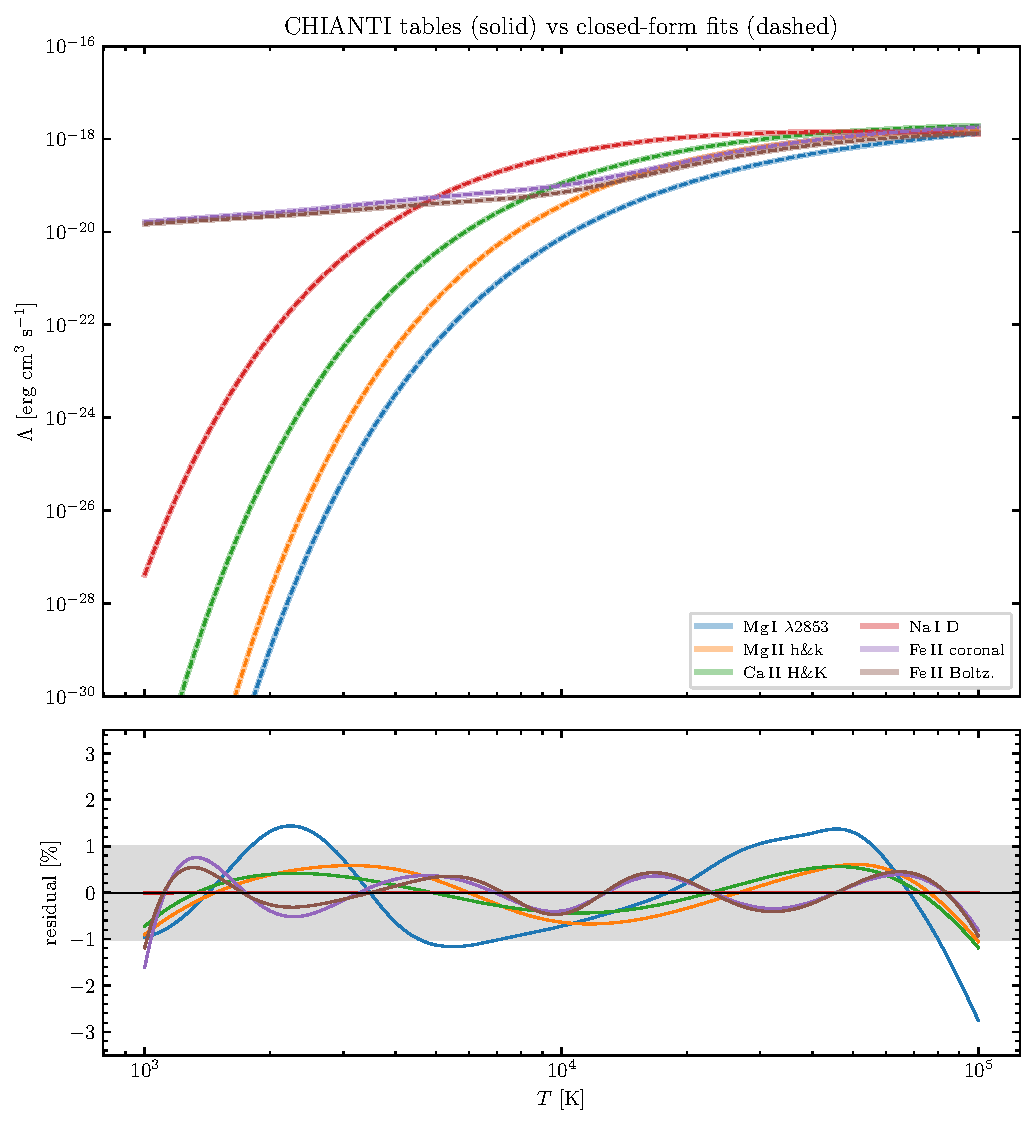
\includegraphics[width=0.78\textwidth]{figures/cool_resonance_fits.pdf}
\caption{CHIANTI cooling tables (solid) vs.\ the closed-form fits
(dashed) for the four resonance channels and the two Fe\,II population
models (Sect.~\ref{sec:feii}).  Bottom: signed residuals; the grey band
is $\pm1\%$.}
\label{fig:resfits}
\end{figure}

\section{Helium: ground-state collisional excitation}
\label{sec:helium}

He\,\textsc{i} and He\,\textsc{ii} are fitted with the same
Eqs.~(\ref{eq:twolevel}--\ref{eq:btups}) as the resonance lines, but the
quantity fitted is a \emph{sum} over every transition out of the ground
level rather than one line.  A single two-level form still works because
the lowest channel sets the temperature dependence: leaving $\Delta E$
free returns $19.88$~eV for He\,\textsc{i} and $40.76$~eV for
He\,\textsc{ii}, each within $0.3\%$ of the lowest level of that ion
($2^3S$ at $19.82$~eV; $n=2$ at $40.81$~eV).

These two coolants were previously represented by expressions inherited
from the ATES lineage that had never been checked against a line list.
The check matters only for helium-rich gas: in a hydrogen-rich wind
Lyman-$\alpha$ exceeds both by orders of magnitude, whereas in a
helium-dominated wind these are the line cooling
(\texttt{helium\_cooling\_channels.tex}).  Two results are worth
recording.  The old He\,\textsc{i} expression,
$1.1\times10^{-19}T^{0.082}e^{-2.3\times10^5/T}$, is a fair
representation of the full ground-state sum despite carrying the
threshold of the lowest channel only --- it is low by $5$--$19\%$ over
$5\times10^3$--$5\times10^4$~K, whereas it differs from the $2^3S$
channel by itself by up to a factor $3.4$.  The old He\,\textsc{ii}
expression is low by a factor of two and gets worse as the temperature
rises.

\begin{table}[htbp]
\centering\small
\caption{Helium ground-state collisional-excitation cooling:
Eqs.~(\ref{eq:twolevel}--\ref{eq:btups}) fitted to the CHIANTI~v11 sum
over all transitions out of the ground level.  ``Max err'' is against
that sum over the fit range; the last column is the error of the
expression each fit replaces, over the range where that coolant can
matter ($5\times10^3$--$5\times10^4$~K for He\,\textsc{i},
$2\times10^4$--$10^5$~K for He\,\textsc{ii}).}
\label{tab:helium}
\begin{tabular}{lccccccc}
\toprule
channel & $g_l$ & $\Delta E$ [eV] & $a$ & $b$ & $T_0$ [K]
        & max err & previous \\
\midrule
He\,\textsc{i} ground sum  & 1 & 19.8843 & 0.0613017 & 0.419181
  & 98213.9 & 1.2\% & $-19.4\%$ \\
He\,\textsc{ii} ground sum & 2 & 40.7562 & 0.437142  & 0.605106
  & 190558.5 & 0.5\% & $-53.6\%$ \\
\bottomrule
\end{tabular}
\end{table}

Written out with the constants collapsed, so that
$\Lambda = C\,T^{-1/2}\,[a + b\ln(1+T/T_0)]\,e^{-T_{\rm ex}/T}$:
%
\begin{align}
\Lambda_{\rm He\,I}(T) &= \frac{2.749039\times10^{-16}}{\sqrt{T}}
  \left[0.0613017 + 0.419181\ln\!\left(1+\frac{T}{9.82139\times10^{4}}\right)\right]
  e^{-230747.5/T}, \\
\Lambda_{\rm He\,II}(T) &= \frac{2.817309\times10^{-16}}{\sqrt{T}}
  \left[0.437142 + 0.605106\ln\!\left(1+\frac{T}{1.90559\times10^{5}}\right)\right]
  e^{-472956.0/T}.
\end{align}

\begin{figure}[htbp]
\centering
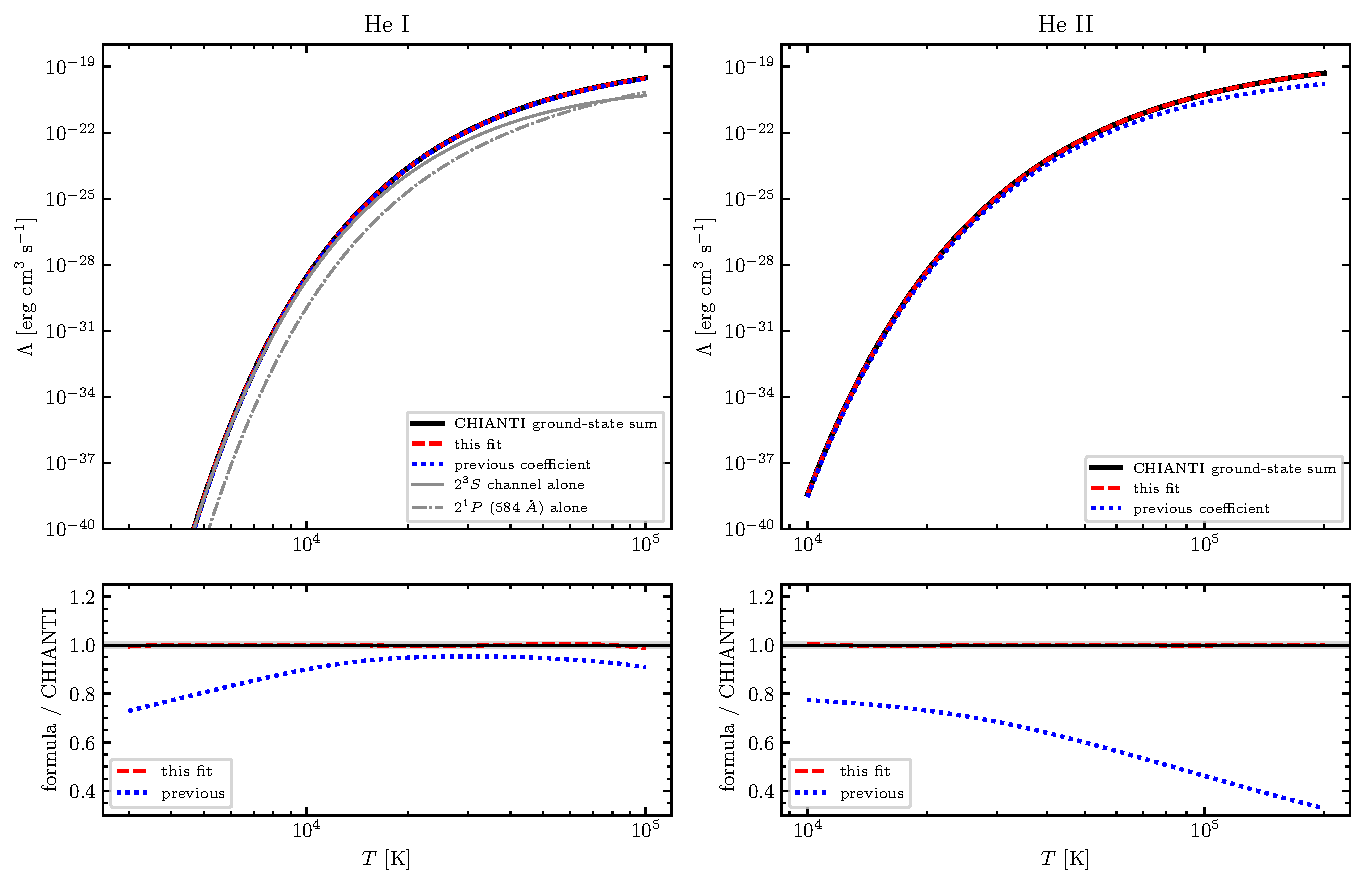
\includegraphics[width=0.92\textwidth]{figures/cool_helium_fits.pdf}
\caption{Helium ground-state collisional-excitation cooling: CHIANTI sum
(solid black), the fits of Table~\ref{tab:helium} (red dashed) and the
expressions they replace (blue dotted).  For He\,\textsc{i} the two
individual channels most often named are shown in grey: the metastable
$2^3S$ channel that sets the exponent, and the $584$~\AA{} resonance
line, which stays well below the total at wind temperatures.  Bottom:
ratio to the CHIANTI sum, with a $\pm1\%$ grey band.}
\label{fig:helium}
\end{figure}

Both fits are optically thin and assume the low-density limit, in which
every collisional excitation is followed by an escaping radiative decay.
Two effects push the true cooling below them in a helium-rich wind: the
$584$~\AA{} line belongs to the dominant species and can be optically
thick, and the $2^3S$ channel feeds a metastable level that the code
tracks separately when the triplet is switched on.  The ground-to-triplet
excitation is inside this term, which is why it is left out of the
triplet system, so that it is not counted twice.

\section{Fe II: sum of effective two-level groups}
\label{sec:feii}

Fe\,II cooling sums hundreds of transitions with $\Delta E$ from
${\sim}0.05$\,eV (a$^6$D fine structure) to several eV, so a single
exponential cannot represent it.  Four effective two-level groups do:
\begin{equation}
\Lambda(T) \;=\; T^{-1/2}\sum_{i=1}^{4} A_i\,e^{-T_i/T}.
\label{eq:multiexp}
\end{equation}
The fitted $T_i$ (Table~\ref{tab:feii}) map onto physically meaningful
transition groups --- infrared fine structure, optical metastable, UV
resonance, and a high-energy tail (Fig.~\ref{fig:feiidecomp}).

\begin{table}[htbp]
\centering\small
\caption{Fe\,II coefficients for Eq.~(\ref{eq:multiexp}).  ``Coronal''
populates the ground level only; ``Boltzmann'' distributes the lower
levels over the metastable manifold ($E<4.8$\,eV, Huang 2023).}
\label{tab:feii}
\begin{tabular}{lcccc}
\toprule
 & \multicolumn{2}{c}{Fe\,II coronal (max err 1.6\%)} &
   \multicolumn{2}{c}{Fe\,II Boltzmann (max err 1.2\%)} \\
\cmidrule(lr){2-3}\cmidrule(lr){4-5}
$i$ & $A_i$ & $T_i$ [K] & $A_i$ & $T_i$ [K] \\
\midrule
1 & $1.9889\times10^{-18}$ & 1350.1   & $1.5019\times10^{-18}$ & 1175.7 \\
2 & $1.6793\times10^{-17}$ & 9630.3   & $9.7419\times10^{-18}$ & 8678.5 \\
3 & $6.5362\times10^{-16}$ & 58939.3  & $5.2485\times10^{-16}$ & 57594.7 \\
4 & $7.4638\times10^{-16}$ & 139593.3 & $4.7387\times10^{-16}$ & 140620.2 \\
\bottomrule
\end{tabular}
\end{table}

\begin{figure}[htbp]
\centering
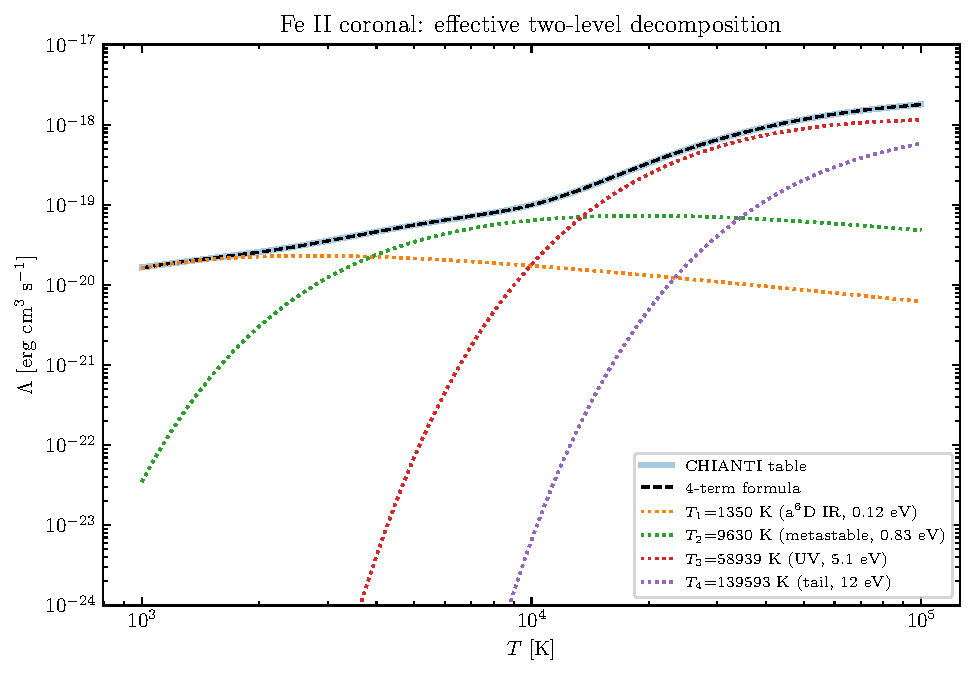
\includegraphics[width=0.62\textwidth]{figures/cool_feii_decomp.pdf}
\caption{Fe\,II coronal cooling decomposed into the four effective
two-level groups of Eq.~(\ref{eq:multiexp}).}
\label{fig:feiidecomp}
\end{figure}

In the cooling \emph{assembly} the coronal formula is superseded by the
2-D statistical-equilibrium table $\Lambda_{\rm eff}(T,n_e)$
(\texttt{cool\_logL\_FeII\_ne}): the forbidden a$^6$D lines have
$n_{\rm crit}\sim10^4$--$10^7\,\mathrm{cm^{-3}}$ and saturate at the
dense base.  The closed-form coronal expression is retained for the
post-process scalar fallback and matches the low-$n_e$ edge of the 2-D
table to ${\sim}1.6\%$.

\section{C, N, O: CHIANTI fits vs.\ the AIOLOS formulas}
\label{sec:cno}

The C/N/O coolants inherited from AIOLOS (\texttt{photochem.cpp}; no
in-code citation, likely Cloudy-calibrated) are
\begin{align}
\Lambda_{\rm CI}^{\rm AIO}  &= 10^{-24} + 3.1\times10^{-20}\,
   e^{-15162/T}\bigl[1+(T/2\times10^4)^{1.5}\bigr],\nonumber\\
\Lambda_{\rm CII}^{\rm AIO} &= 1.5\times10^{-23} + 3.1\times10^{-20}\,
   e^{-45162/T}\bigl[1+(T/7500)^{1.5}\bigr],\nonumber\\
\Lambda_{\rm OI}^{\rm AIO}  &= 5.5\times10^{-24} + 1.1\times10^{-20}\,
   e^{-30162/T}\bigl[1+(T/7500)^{0.5}\bigr],\nonumber\\
\Lambda_{\rm OII}^{\rm AIO} &= 5.1\times10^{-20}\,
   e^{-35162/T}\bigl[1+(T/7500)^{0.5}\bigr],
\label{eq:aiolos}
\end{align}
with no nitrogen cooling at all.  The replacement CHIANTI fits use the
same multi-exponential form as Fe\,II,
Eq.~(\ref{eq:multiexp}) with 4--6 terms (Table~\ref{tab:cno}); lower
levels are Boltzmann-populated over the ground-term fine structure
(C\,I\,$^3$P, C\,II\,$^2$P, N\,II\,$^3$P, O\,I\,$^3$P; the $^4$S
ground of N\,I and O\,II is a single level).

Figure~\ref{fig:cno} compares the three.  The AIOLOS carbon fits track
CHIANTI remarkably well near $10^4$\,K (C\,I to ${\sim}1\%$), which
suggests they were calibrated against data of similar provenance; the
oxygen fits however deviate by 40--70\% across the wind-launch region
($1$--$3\times10^4$\,K), and nitrogen --- a non-negligible coolant
around $2\times10^4$\,K --- was absent entirely.  The runtime key
\texttt{cno\_cool} in \texttt{metals.inp} selects the source
(\texttt{1} = CHIANTI fits, the default; \texttt{0} = AIOLOS).

\begin{table}[htbp]
\centering\small
\caption{C/N/O coefficients for Eq.~(\ref{eq:multiexp}) (CHIANTI
ground-term curves; per $(n_e n_{\rm ion})$).  The notation $a(b)$
means $a\times10^{b}$.  Max err is vs.\ the recomputed CHIANTI curve
over $10^3$--$10^5$\,K.}
\label{tab:cno}
\begin{tabular}{llcccccc}
\toprule
ion (max err) & & $i{=}1$ & $i{=}2$ & $i{=}3$ & $i{=}4$ & $i{=}5$ & $i{=}6$ \\
\midrule
C\,I (1.8\%)  & $A_i$ & 1.106($-$20) & 1.392($-$18) & 6.962($-$18) & 6.593($-$17) & 3.017($-$16) & \\
              & $T_i$ [K] & 2351 & 15172 & 25411 & 72609 & 177264 & \\
\addlinespace[2pt]
C\,II (0.5\%) & $A_i$ & 3.004($-$20) & 2.410($-$20) & 3.904($-$17) & 3.332($-$16) & 1.360($-$15) & \\
              & $T_i$ [K] & 61.4 & 7183 & 64104 & 124809 & 246136 & \\
\addlinespace[2pt]
N\,I (0.6\%)  & $A_i$ & 1.514($-$18) & 4.877($-$18) & 1.160($-$17) & 1.575($-$16) & 3.175($-$16) & \\
              & $T_i$ [K] & 29686 & 34694 & 50741 & 139916 & 254192 & \\
\addlinespace[2pt]
N\,II (0.1\%) & $A_i$ & 2.406($-$20) & 1.244($-$20) & 8.040($-$18) & 1.545($-$17) & 2.884($-$16) & 6.944($-$16) \\
              & $T_i$ [K] & 49.9 & 6521 & 23771 & 64487 & 157103 & 295894 \\
\addlinespace[2pt]
O\,I (2.1\%)  & $A_i$ & 3.236($-$22) & 6.572($-$20) & 1.803($-$18) & 6.762($-$18) & 3.372($-$17) & \\
              & $T_i$ [K] & 848 & 19059 & 31568 & 70528 & 178827 & \\
\addlinespace[2pt]
O\,II (0.2\%) & $A_i$ & 1.768($-$17) & 8.071($-$18) & 2.344($-$16) & 8.789($-$16) & & \\
              & $T_i$ [K] & 44129 & 59732 & 179091 & 325669 & & \\
\bottomrule
\end{tabular}
\end{table}

\begin{figure}[htbp]
\centering
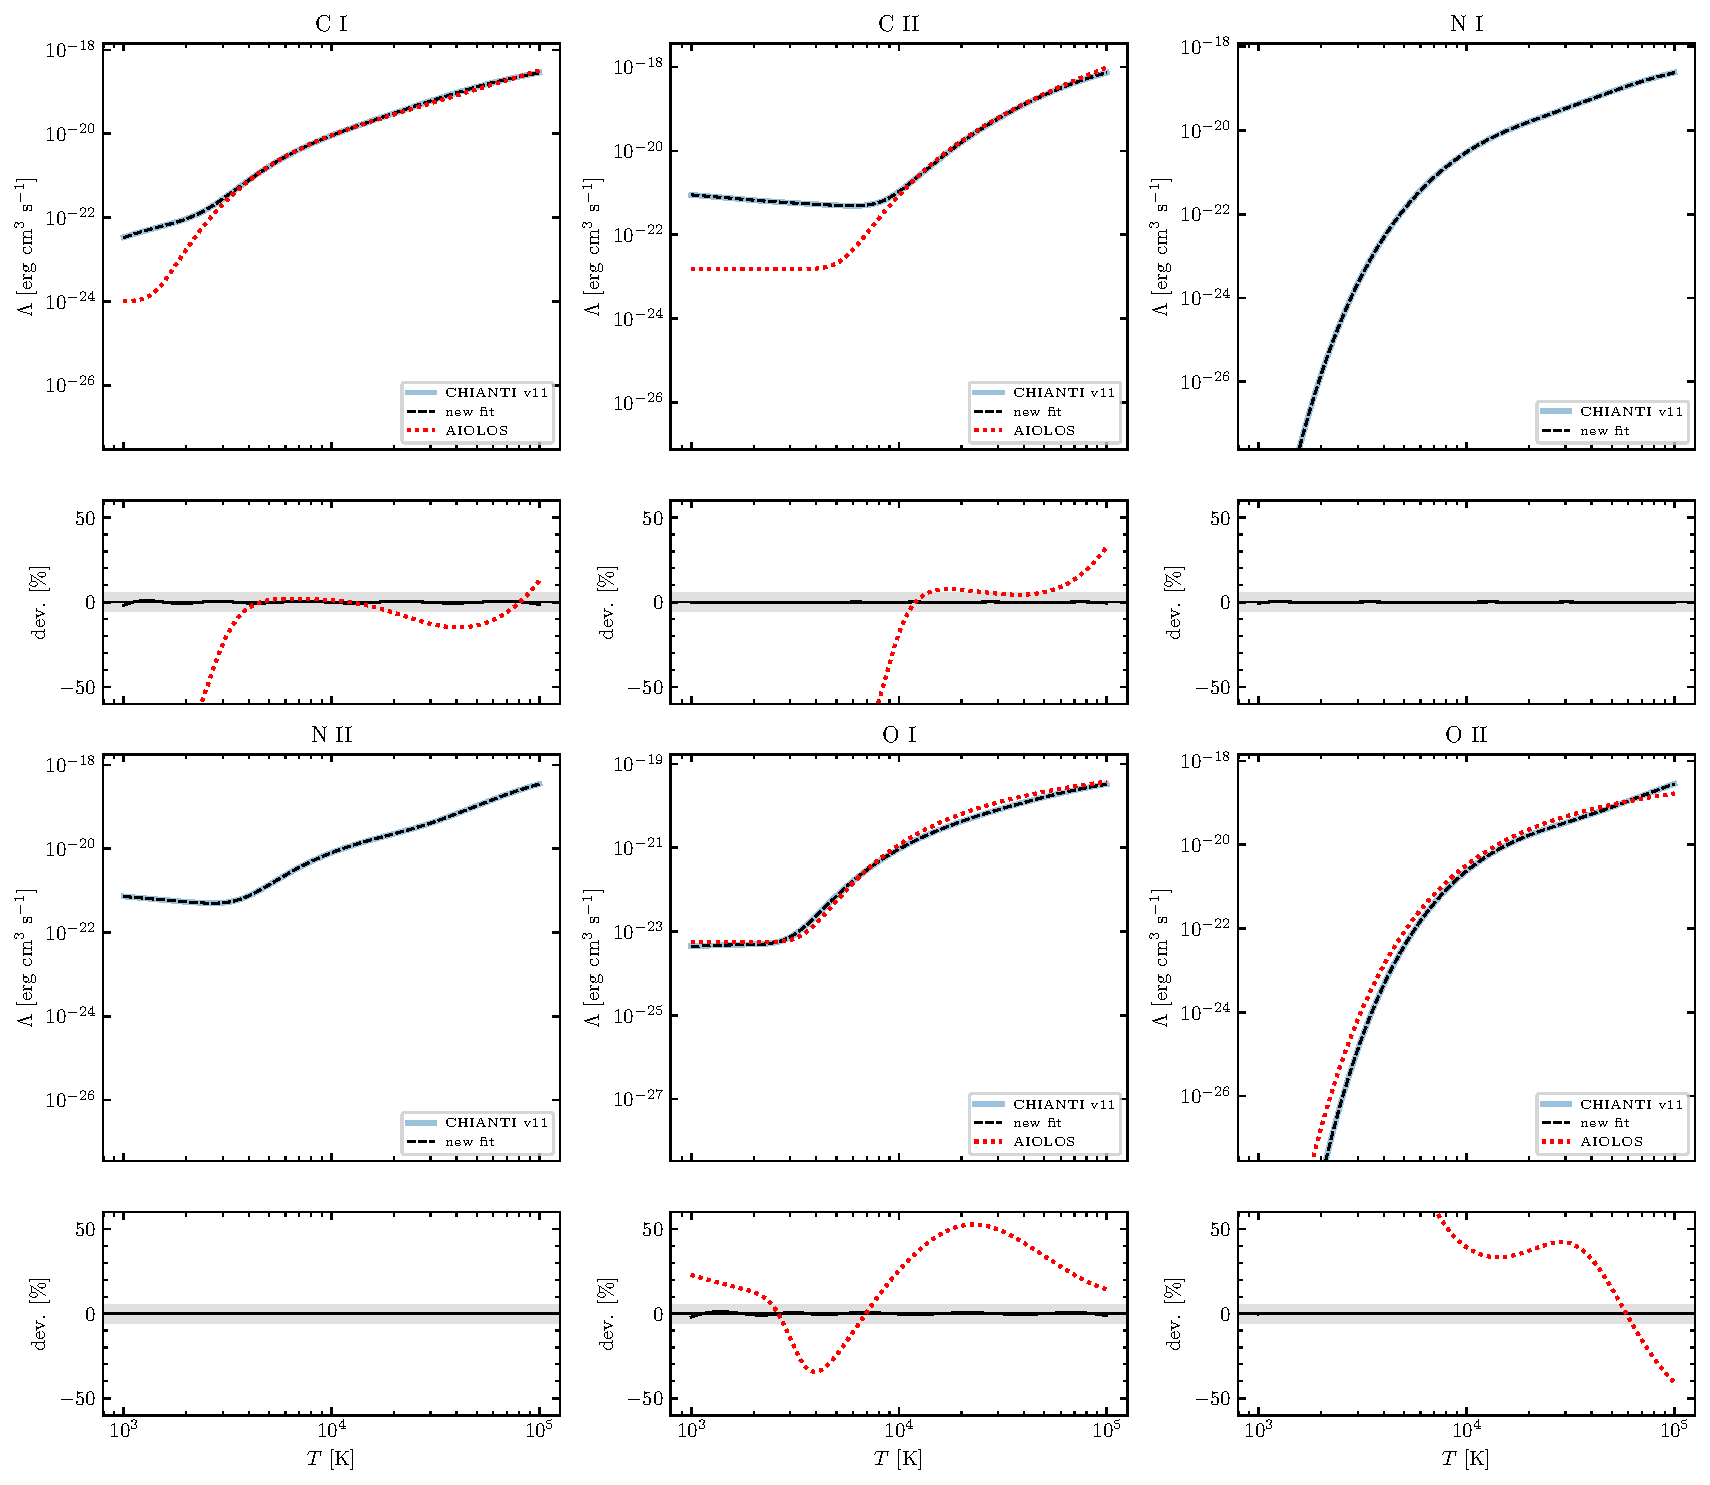
\includegraphics[width=0.92\textwidth]{figures/cool_cno_compare.pdf}
\caption{C/N/O line cooling: CHIANTI v11 (solid blue), the new
closed-form fits (black dashed), and the AIOLOS formulas (red
dotted; absent for nitrogen).  Deviation strips show the percentage
difference from CHIANTI; the grey band is $\pm5\%$.}
\label{fig:cno}
\end{figure}

\section{Ground-term fine-structure statistical equilibrium}
\label{sec:fs}

The coronal C/N/O curves carry the ground-term fine-structure (FS) lines
in the optically thin, \emph{low-density} limit, although their critical
densities are of order $10^0$--$10^5\,\mathrm{cm^{-3}}$, decades below
the base density of an irradiated atmosphere
($n_e\sim10^9$, $n_{\rm HI}\sim10^{14}\,\mathrm{cm^{-3}}$).  At the
converged base of the four planet runs the coronal form overshoots what
the same lines can actually radiate by 2.9--8.3 decades
(Table~\ref{tab:fsover}).  In the CHIANTI mode the FS part is therefore
replaced, for every C/N/O coolant whose ground term is split, by the
exact statistical-equilibrium (SE) solution of that term,
\begin{equation}
\sum_j f_j R_{ji} = f_i \sum_j R_{ij},\qquad \sum_i f_i = 1,
\label{eq:se}
\end{equation}
\begin{equation}
R_{ul} = C_{ul} + \beta_{ul} A_{ul},\qquad
R_{lu} = C_{ul}\,\frac{g_u}{g_l}\,e^{-E_{ul}/k_BT},\qquad
C_{ul} = n_e k_{e,ul}(T) + n_{\rm HI}\,k_{{\rm H},ul}(T),
\end{equation}
\begin{equation}
W_{\rm FS} = \sum_{u>l} f_u\,\beta_{ul}A_{ul}\,k_B E_{ul}
\qquad [\mathrm{erg\,s^{-1}}\ \mathrm{per\ ion}],
\label{eq:wfs}
\end{equation}
together with a multi-exponential refit $\Lambda_{\rm rem}(T)$ of the
CHIANTI curve that keeps \emph{only} the channels leaving the ground
term.  The assembly uses
$\Lambda_{\rm eff} = W_{\rm FS}/n_e + \Lambda_{\rm rem}(T)$, so the
$n_e$ prefactor cancels and the H-collision channel --- which the
electron-only coronal curves lack entirely --- is recovered exactly.
The ions treated are the complete set of split ground terms among the
coolants:

\begin{center}
\begin{tabular}{llll}
\hline
ion & ground term & levels & lines \\
\hline
C\,I  & $2p^2\ ^3P_{0,1,2}$   & 3 & [C\,I] 609.1, 370.4\,$\mu$m \\
C\,II & $2p\ ^2P_{1/2,3/2}$   & 2 & [C\,II] 157.7\,$\mu$m \\
N\,II & $2p^2\ ^3P_{0,1,2}$   & 3 & [N\,II] 205.3, 121.8\,$\mu$m \\
O\,I  & $2p^4\ ^3P_{2,1,0}$   & 3 & [O\,I] 63.2, 145.5, 44.1\,$\mu$m \\
\hline
\end{tabular}
\end{center}

\noindent
N\,I and O\,II have a single-level $^4S$ ground term; Mg\,I/II, Ca\,II
and Na\,I have a single ground level; Fe\,I is built from permitted
lines only; and Fe\,II is already density-dependent through its
two-dimensional SE table (Section~\ref{sec:feii}).  The $^3P_2$--$^3P_0$
channels of C\,I and N\,II have no CHIANTI transition probability
(magnetic quadrupole, $A<10^{-12}\,\mathrm{s^{-1}}$) and enter as
collisional couplings only.

\paragraph{Limits.}  As $n_e,n_{\rm HI}\to0$ the SE populations collapse
onto the ground level and Eq.~(\ref{eq:wfs}) reproduces the coronal
within-term channel to the accuracy of the $\Upsilon$ fits (1.3--4.4\%).
As either density $\to\infty$ it saturates at the exact multilevel LTE
emission $\sum_u f_u^{\rm Boltz} A_{ul} h\nu_{ul}$, verified to
$10^{-14}$ relative.  The earlier two-level treatment of [O\,I]
63\,$\mu$m and [C\,II] 158\,$\mu$m multiplied a two-level solution ---
already normalized to the \emph{two-level} partition function --- by the
ground-term Boltzmann fraction of its lower level; that double
normalization left its LTE limit low by a factor
$1+(g_u/g_l)e^{-E/k_BT}$, i.e.\ $2.7\times$ for [C\,II] 158\,$\mu$m at
the 530\,K base of HD\,189733\,b.  $\Lambda_{\rm rem}$ keeps the
ground-term Boltzmann weighting of its lower levels, the convention of
the CHIANTI curves it is fitted to; that is the right weighting wherever
it matters, and where it is not the ground-only and Boltzmann weightings
agree to 1.4--1.9\% anyway, because $\Upsilon_{lu}\propto g_l$ for the
LS-coupled transitions that leave the ground term.

\paragraph{Line trapping.}  $\beta_{ul}$ is the escape probability of
that FS line and enters as $A_{ul}\to\beta_{ul}A_{ul}$ \emph{inside}
Eq.~(\ref{eq:se}), not as a factor on Eq.~(\ref{eq:wfs}).  That is the
physically correct place: in the subcritical limit the cooling is set by
the collisional excitation rate and is independent of $\beta$, while in
the saturated limit the escaping flux is proportional to $\beta$.
The functional form is the Doppler-core single-flight escape probability
of Hollenbach \& McKee (1979) and de Jong, Boland \& Dalgarno (1980),
per face,
\begin{equation}
\beta_1(\tau) \;=\;
\begin{cases}
  \dfrac{1-e^{-a\tau}}{2a\tau}, & \tau < \tau_c,\\[8pt]
  \dfrac{1}{4\tau\sqrt{\ln\!\left(\tau/\sqrt{\pi}\right)}}, & \tau \ge \tau_c,
\end{cases}
\qquad a = 2.34,
\label{eq:beta1}
\end{equation}
with $\tau$ the line-center optical depth from the cell to that face;
the two branches meet continuously in value at
$\tau_c=\sqrt{\pi}\,e^{a^2/4}\simeq 6.97$ (the residual slope kink there
is below 1\%), and $\beta_1(0)=1/2$ --- half of the photons leave through
the near face.  The escape probability of a cell is the two-face sum,
$\beta_{ul}=\beta_1(\tau_{\rm up})+\beta_1(\tau_{\rm dn})$
(\texttt{line\_escape\_probability\_one\_face},
\texttt{Cool\_coeff.f90}); with \texttt{Base IR field} on, the downward
face also carries the blackbody photon occupation number of the
atmosphere below (\texttt{docs/lower\_atmosphere\_coupling}).  The
opacity of each line uses the same atomic data and the ground-term
Boltzmann lower-level population.  $\Lambda_{\rm rem}$ is left optically
thin.

\paragraph{Atomic data.}  Levels, $A$ values and the electron collision
strengths are CHIANTI v11.0.2 (\texttt{elvlc} / \texttt{wgfa} /
\texttt{scups}); $\log_{10}\Upsilon$ is a quartic in
$x=\log_{10}(T/10^4)$ fitted over $10^3$--$10^5$\,K (max error 4.8\%,
against 8.8\% for a cubic on the C\,I $^3P_0$--$^3P_2$ strength) and
$T$ is clamped to that range.  The electron de-excitation rate is
$k_e = 8.629\times10^{-6}\,\Upsilon(T)/(g_u\sqrt T)$.  The H-atom
de-excitation rates are taken from quantum scattering calculations,
$\log_{10}k_{\rm H}$ a quadratic in $\log_{10}(T/10^3)$ with $T$ clamped
to the tabulated range (max error 4.9\%):

\begin{center}
\begin{tabular}{lll}
\hline
ion & source & range \\
\hline
C\,I, N\,II & Yan \& Babb (2023), MNRAS 518, 6004, Tables 1--2 & 10--$10^4$\,K \\
O\,I  & Abrahamsson, Krems \& Dalgarno (2007), ApJ 654, 1171 & 20--1000\,K \\
C\,II & Barinovs et al.\ (2005), ApJ 620, 537 & 20--2000\,K \\
\hline
\end{tabular}
\end{center}

\noindent
These replace the values of the legacy \texttt{use\_2lev\_cool} branch
(a constant $4.0\times10^{-11}$ for [C\,II] 158\,$\mu$m$+$H and
$4.2\times10^{-11}(T/100)^{0.67}$ for [O\,I] 63\,$\mu$m$+$H, both
flagged approximate), which are 5--20$\times$ below them.  H collisions
on the \emph{ion} N\,II are included on the same footing as on the
neutrals; they are not what saturates N\,II at the base
($n_{\rm crit,e}$ of [N\,II] 205\,$\mu$m is ${\sim}10^2\,\mathrm{cm^{-3}}$),
they matter only in gas thin enough for the electron channel alone to be
subcritical.  \texttt{cooling\_data/fit\_fs\_saturation.py} is the
auditable source and prints every coefficient.

\begin{table}[htbp]
\centering
\caption{Ground-term fine-structure cooling at the converged base cell of
each run: the coronal within-term channel as the CHIANTI fits carry it,
against the exact SE value at the local $(n_e,n_{\rm HI})$, both
volumetric [erg\,cm$^{-3}$\,s$^{-1}$], $\beta=1$.  The last column is the
SE value as a fraction of the local heating rate.}
\label{tab:fsover}
\begin{tabular}{llrrrr}
\hline
run & ion & coronal & SE (saturated) & decades & SE/heat \\
\hline
HD\,189733\,b   & C\,I  & $1.61\times10^{-4}$ & $2.00\times10^{-11}$ & 6.9 & $5.9\times10^{-6}$\\
$T=528$\,K      & C\,II & $1.14\times10^{-4}$ & $2.09\times10^{-12}$ & 7.7 & $6.2\times10^{-7}$\\
                & N\,II & $7.47\times10^{-10}$& $5.97\times10^{-17}$ & 7.1 & $1.8\times10^{-11}$\\
                & O\,I  & $1.47\times10^{-4}$ & $3.08\times10^{-8}$  & 3.7 & $9.1\times10^{-3}$\\
\hline
HD\,209458\,b   & C\,I  & $7.77\times10^{-5}$ & $5.76\times10^{-11}$ & 6.1 & $3.0\times10^{-4}$\\
$T=519$\,K      & C\,II & $2.50\times10^{-12}$& $2.56\times10^{-19}$ & 7.0 & $1.3\times10^{-12}$\\
                & N\,II & $1.28\times10^{-15}$& $5.72\times10^{-22}$ & 6.3 & $3.0\times10^{-15}$\\
                & O\,I  & $7.42\times10^{-5}$ & $8.77\times10^{-8}$  & 2.9 & $4.5\times10^{-1}$\\
\hline
WASP-52\,b      & C\,I  & $2.15\times10^{-5}$ & $1.94\times10^{-12}$ & 7.0 & $1.1\times10^{-6}$\\
$T=794$\,K      & C\,II & $6.14\times10^{-5}$ & $2.43\times10^{-12}$ & 7.4 & $1.4\times10^{-6}$\\
                & N\,II & $8.42\times10^{-10}$& $1.48\times10^{-16}$ & 6.8 & $8.2\times10^{-11}$\\
                & O\,I  & $8.92\times10^{-6}$ & $3.40\times10^{-9}$  & 3.4 & $1.9\times10^{-3}$\\
\hline
WASP-121\,b     & C\,I  & $8.08\times10^{-6}$ & $4.48\times10^{-14}$ & 8.3 & $5.2\times10^{-9}$\\
$T=2407$\,K     & C\,II & $8.19\times10^{-4}$ & $1.33\times10^{-11}$ & 7.8 & $1.6\times10^{-6}$\\
                & N\,II & $1.14\times10^{-8}$ & $8.49\times10^{-16}$ & 7.1 & $9.9\times10^{-11}$\\
                & O\,I  & $1.26\times10^{-5}$ & $1.20\times10^{-9}$  & 4.0 & $1.4\times10^{-4}$\\
\hline
\end{tabular}
\end{table}

\begin{figure}[htbp]
\centering
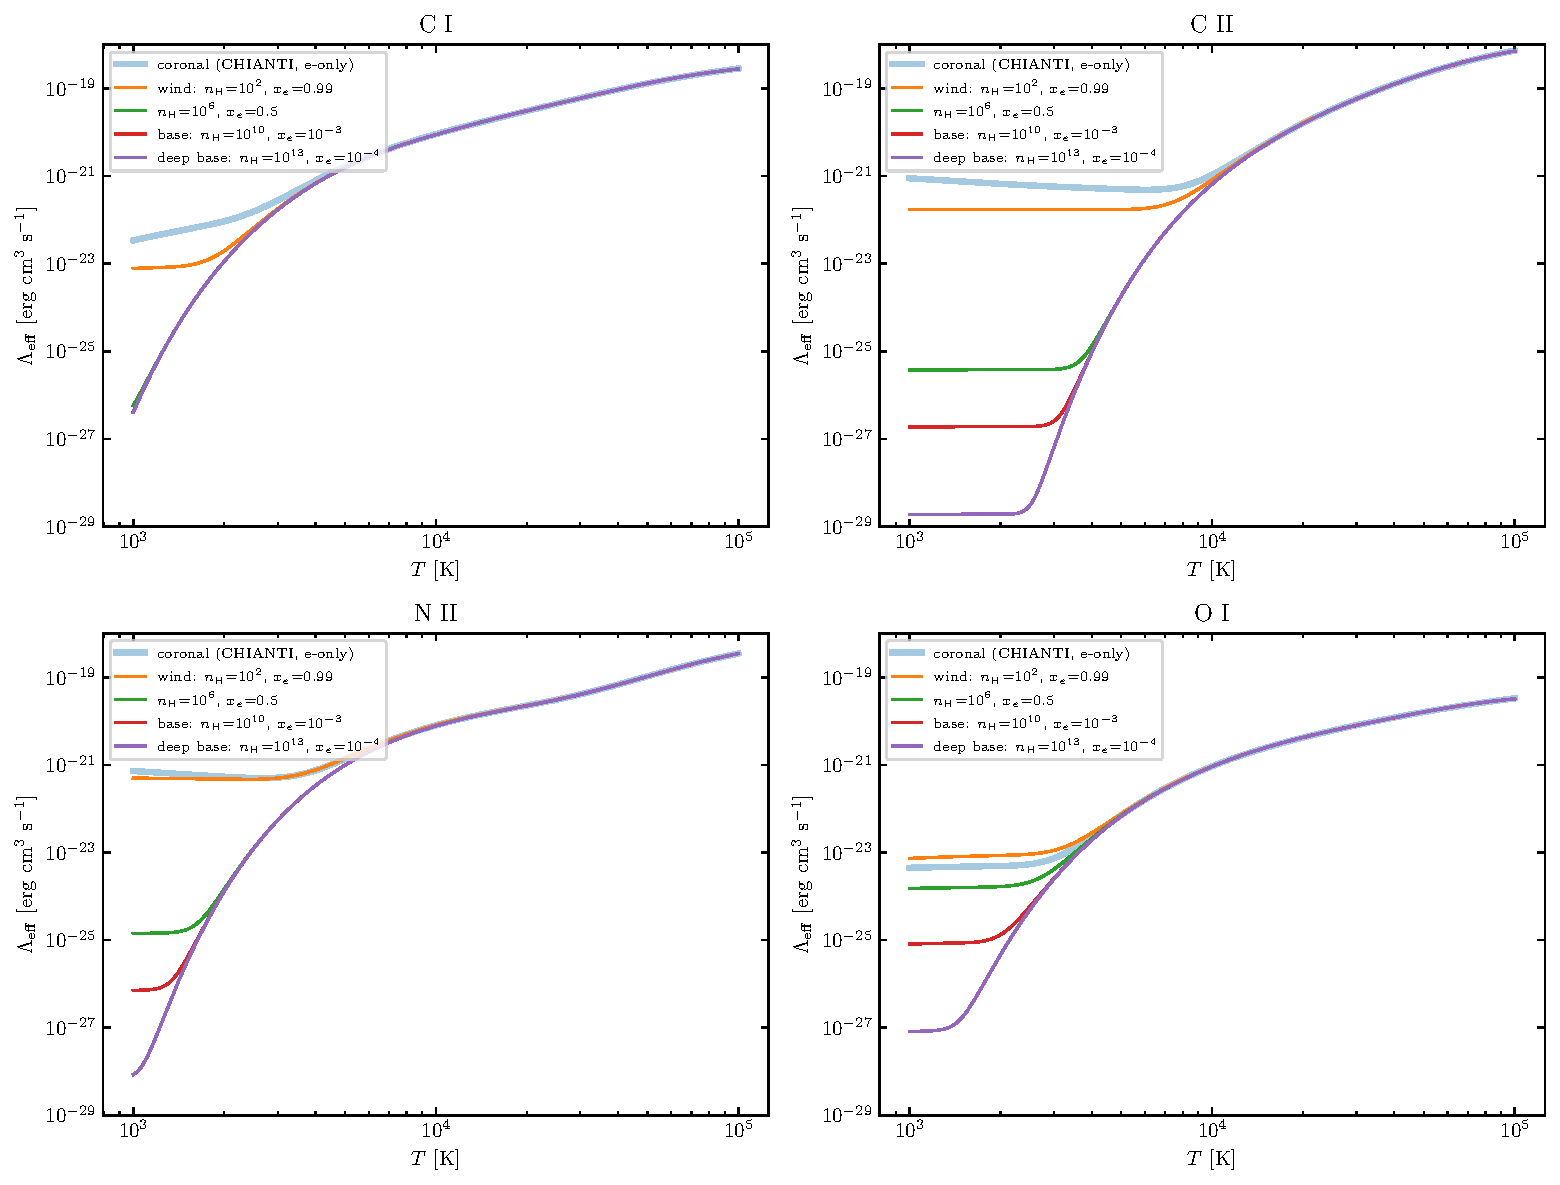
\includegraphics[width=0.95\textwidth]{figures/cool_fs_saturation.pdf}
\caption{Effective C\,I, C\,II, N\,II and O\,I cooling coefficients with
the ground term solved in statistical equilibrium, Eqs.~(\ref{eq:se})
and (\ref{eq:wfs}), for densities from the wind to the deep base,
compared with the electron-only coronal curve.  The low-temperature
plateau of each coronal curve is the unsaturated fine-structure floor;
it collapses by several decades once the ground term is allowed to
thermalise.}
\label{fig:fssat}
\end{figure}

\paragraph{Impact.}  The effect is confined to the base but is not
small there.  On HD\,189733\,b the C\,I coronal floor had been the
dominant coolant of the whole layer below $r\simeq1.01\,R_p$
($3.3\times10^{-6}$ against a local heating of $3.4\times10^{-6}$
erg\,cm$^{-3}$\,s$^{-1}$); with the ground term saturated it falls to
$10^{-11}$, the base warms from 528 to 613\,K, the density at
$1.01\,R_p$ rises by a factor 3.3 and the mass-loss rate at $r=2\,R_p$
increases by 21\%, from $2.35\times10^{9}$ to
$2.85\times10^{9}\,\mathrm{g\,s^{-1}}$.  Outside $r\simeq1.1\,R_p$ the
temperature profile moves by less than 4\%.  The same change also
removes the sensitivity of the base to the coronal-fit cutoff width
$w$: see \texttt{docs/coronal\_cutoff\_width.md}.

\section{Free--free and the remaining tabulated pieces}

Free--free cooling keeps the Huang (2023) Eq.~(9) form,
$\Lambda_{\rm ff} = 1.9095\times10^{-25}\,Z^2\,(T/10^4)^{0.55}$ per
$(n_e n_{\rm ion})$.  Two coefficients remain tabulated because they
are not reducible to closed form: Fe\,I (NIST $f$-values + Van
Regemorter over the even-parity metastable manifold; 1-D in $T$) and
the Fe\,II multilevel statistical-equilibrium coefficient
$\Lambda_{\rm eff}(T,n_e)$ (2-D).  A possible future step, analogous to
Sect.~\ref{sec:fs}, would be a closed-form saturation treatment of the
Fe\,II a$^6$D manifold, but the 2-D table is exact within its grid and
carries no runtime cost concern.

\paragraph{Known limitations.}
(i) The legacy \texttt{use\_2lev\_cool} branch hard-codes the AIOLOS
exponential parts for C\,II/O\,I and is not reached by the CHIANTI
formulas; it is superseded by Sect.~\ref{sec:fs} and kept only for
comparison (default off).
(ii) The H-collision rates of Sect.~\ref{sec:fs} are fits to published
quantum scattering calculations, but O\,I is tabulated only to 1000\,K
and C\,II to 2000\,K; above those the rate is held at its endpoint value
rather than extrapolated.
(iii) All formulas are calibrated over $10^3$--$10^5$\,K; outside this
range they extrapolate smoothly but are unvalidated.

\end{document}
